\documentclass{beamer}
\usepackage{color}
\usepackage{graphicx}

\usepackage[T1]{fontenc}
\usepackage[utf8]{inputenc}
\usepackage[english]{babel}
\usepackage{amsfonts,amsmath,amssymb,amsthm}
\usepackage{alltt}
\usepackage{mathrsfs} 
\usepackage{multicol}
\usepackage{subfigure}
\usepackage{ragged2e}
\usepackage{newtxtext,newtxmath}
\usepackage{multirow}
\usepackage{booktabs}
\usepackage{animate}
\usepackage{makecell}

\usefonttheme{professionalfonts}

\usetheme{cinvestavbokumantle}
\title{High Quality Labeling}
\author{Andrea Elizabeth González Ramírez}

\begin{document}

\begin{frame}
    \titlepage
    \thispagestyle{empty}
\end{frame}

\section{}
\begin{frame}
    \begin{figure}
        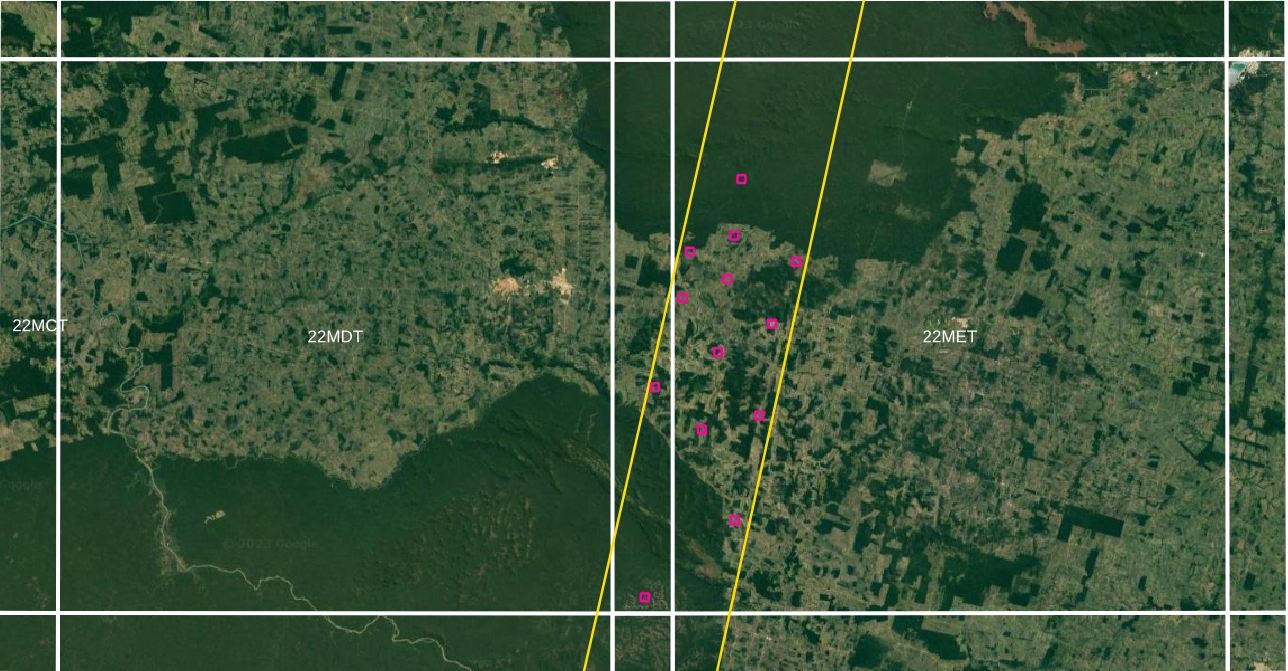
\includegraphics[width=10cm]{Figures/v3/overlaping_polygons_1.png}
        \caption{All polygons over area of interest: 22MET overlap.}  
        \centering
    \end{figure}
\end{frame}

\section{Dataset}
\begin{frame}{Implementation details}
    \begin{minipage}{0.6\textwidth}
        \begin{table}
            \scriptsize
            \begin{tabular}{c|c}
                \hline
                \multicolumn{2}{c}{\textbf{Dataset}} \\
                \hline  	
                Tiles &  22MET \\
                Number of polygons & 11 \\
                Time observation & \makecell{2019-05-01 \\ 2019-09-30} \\
                Visualization of TC images & 0-3000 \\
                \hline
            \end{tabular}
            \caption{Description of the dataset.}
        \end{table}
    \end{minipage}
    \begin{minipage}{0.35\textwidth}
        \begin{table}
            \scriptsize
            \begin{tabular}{c|c}
            \hline
                \multicolumn{2}{c}{\textbf{Classes}} \\ \hline
                Fully Cloudy & FC \\
                Partly Cloudy& PC \\
                Full Shadow & FS \\
                Partly Shadow& PS \\
                Low quality & LQ \\
                Medium quality & MQ\\
                High quality & HQ \\
                \hline
            \end{tabular}
            \caption{Description of the labeling.}
        \end{table}
    \end{minipage}
\end{frame}

\section{Labeling}
\begin{frame}
    \begin{figure}
        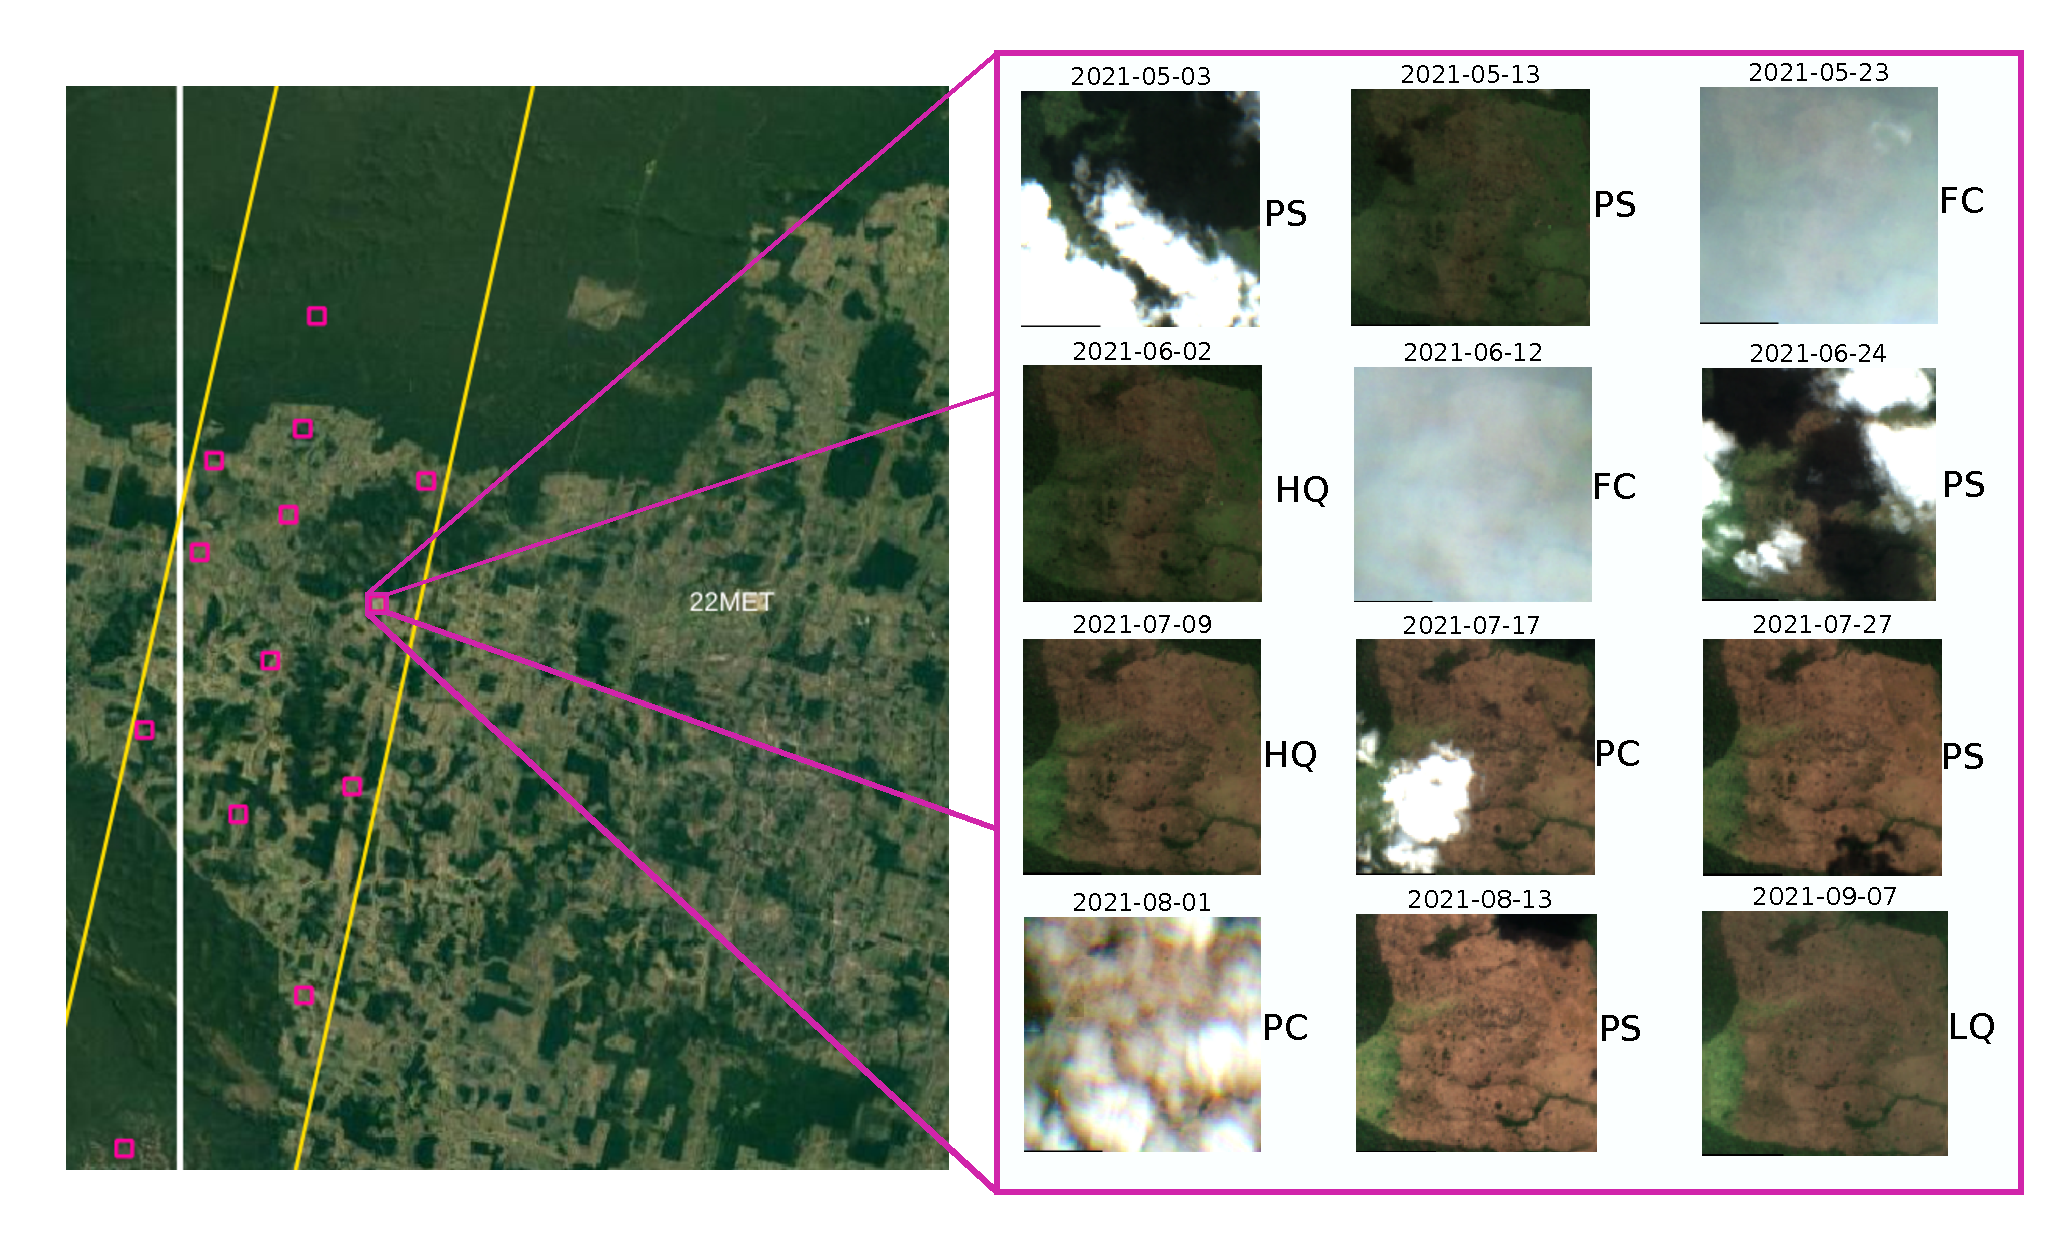
\includegraphics[width=10cm]{Figures/v3/labeling/polygon_0.pdf}
        \caption{Temporal observation of the polygon 0.}  
        \centering
    \end{figure}
\end{frame}

\begin{frame}
    \begin{figure}
        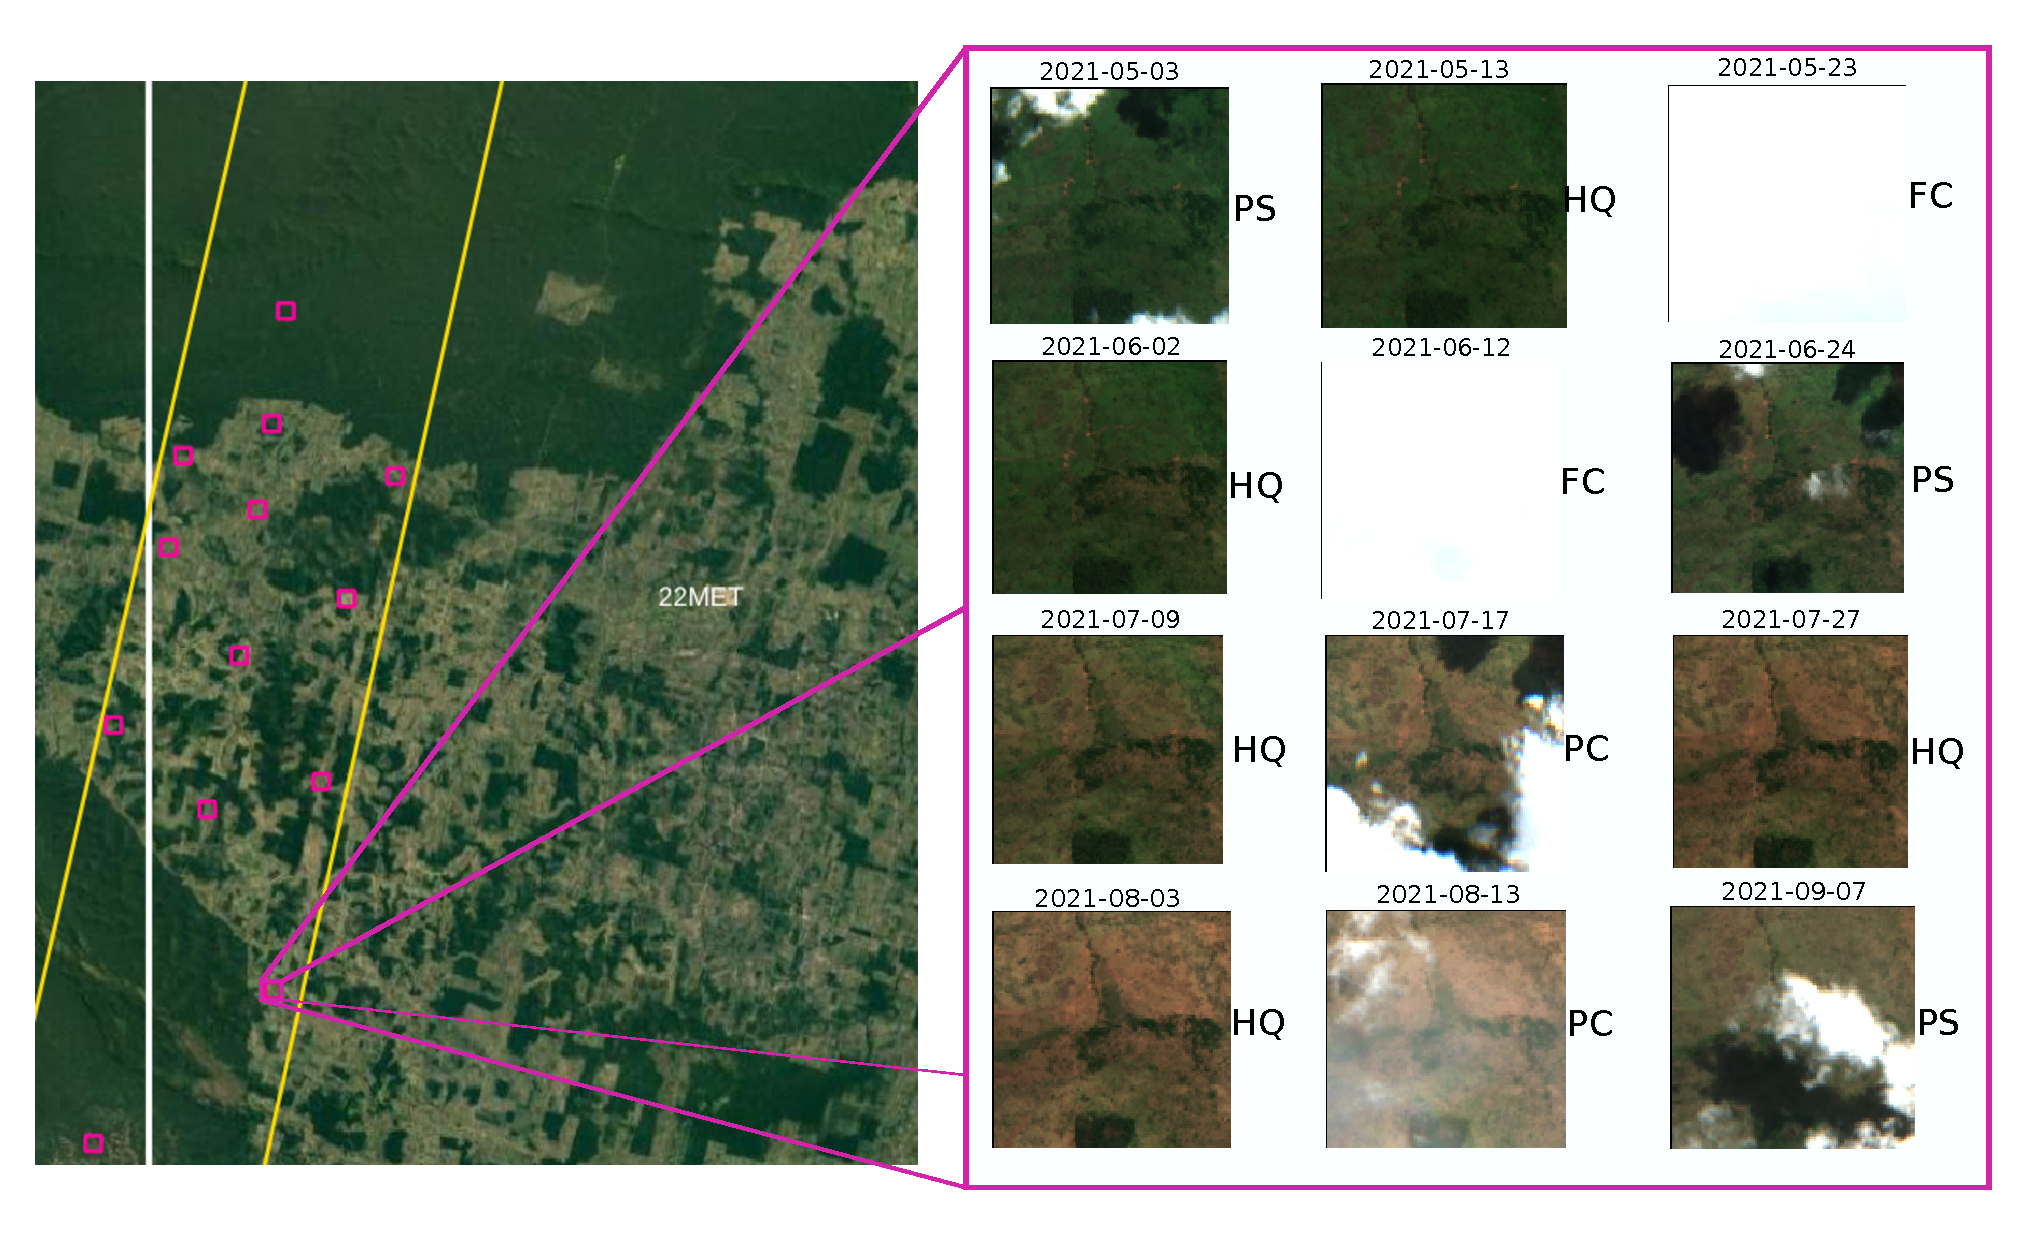
\includegraphics[width=10cm]{Figures/v3/labeling/polygon_2.pdf}
        \caption{Temporal observation of the polygon 2.}  
        \centering
    \end{figure}
\end{frame}

\begin{frame}
    \begin{figure}
        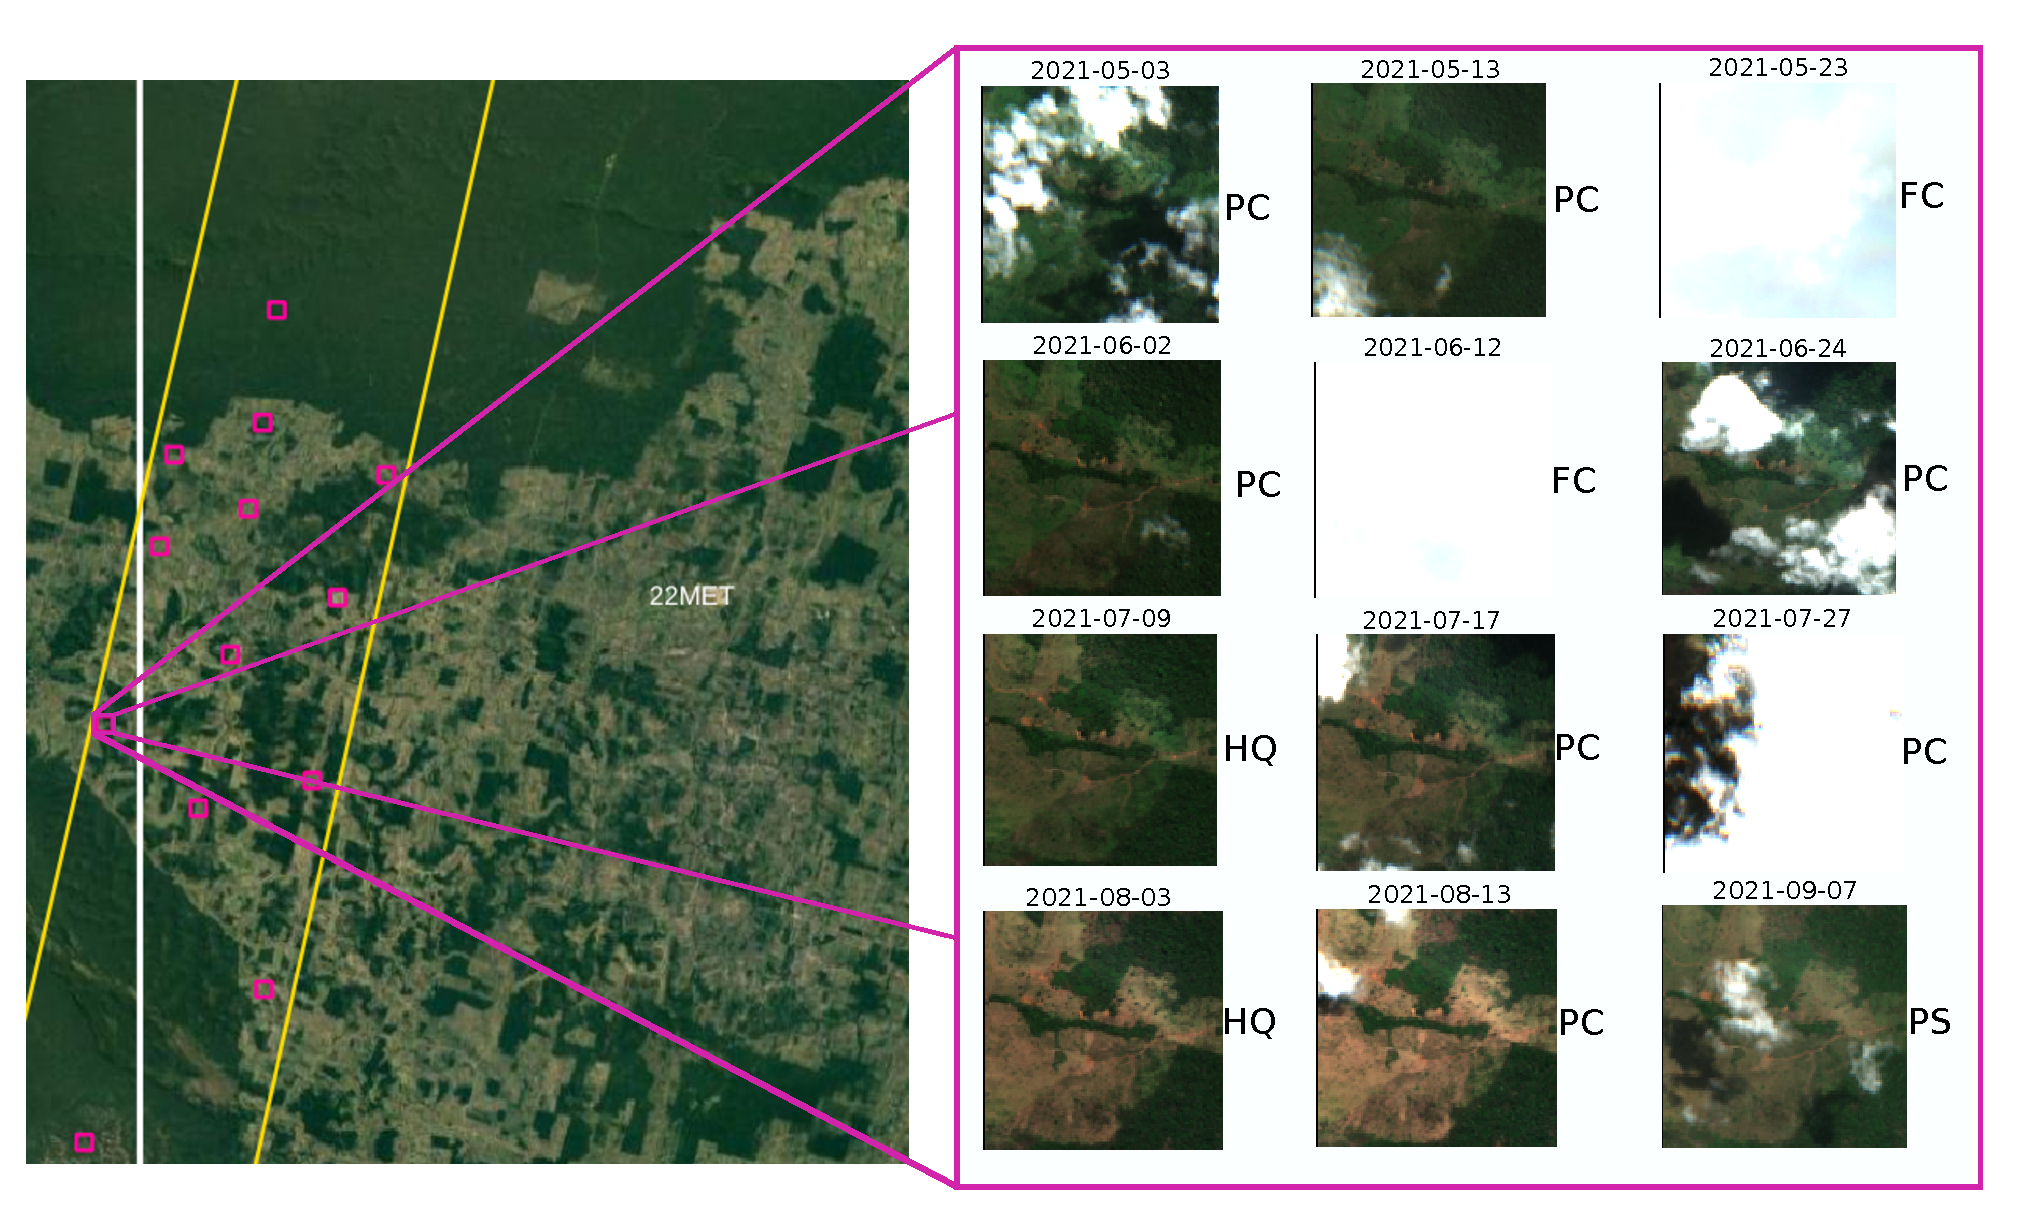
\includegraphics[width=10cm]{Figures/v3/labeling/polygon_4.pdf}
        \caption{Temporal observation of the polygon 4.}  
        \centering
    \end{figure}
\end{frame}

\begin{frame}
    \begin{figure}
        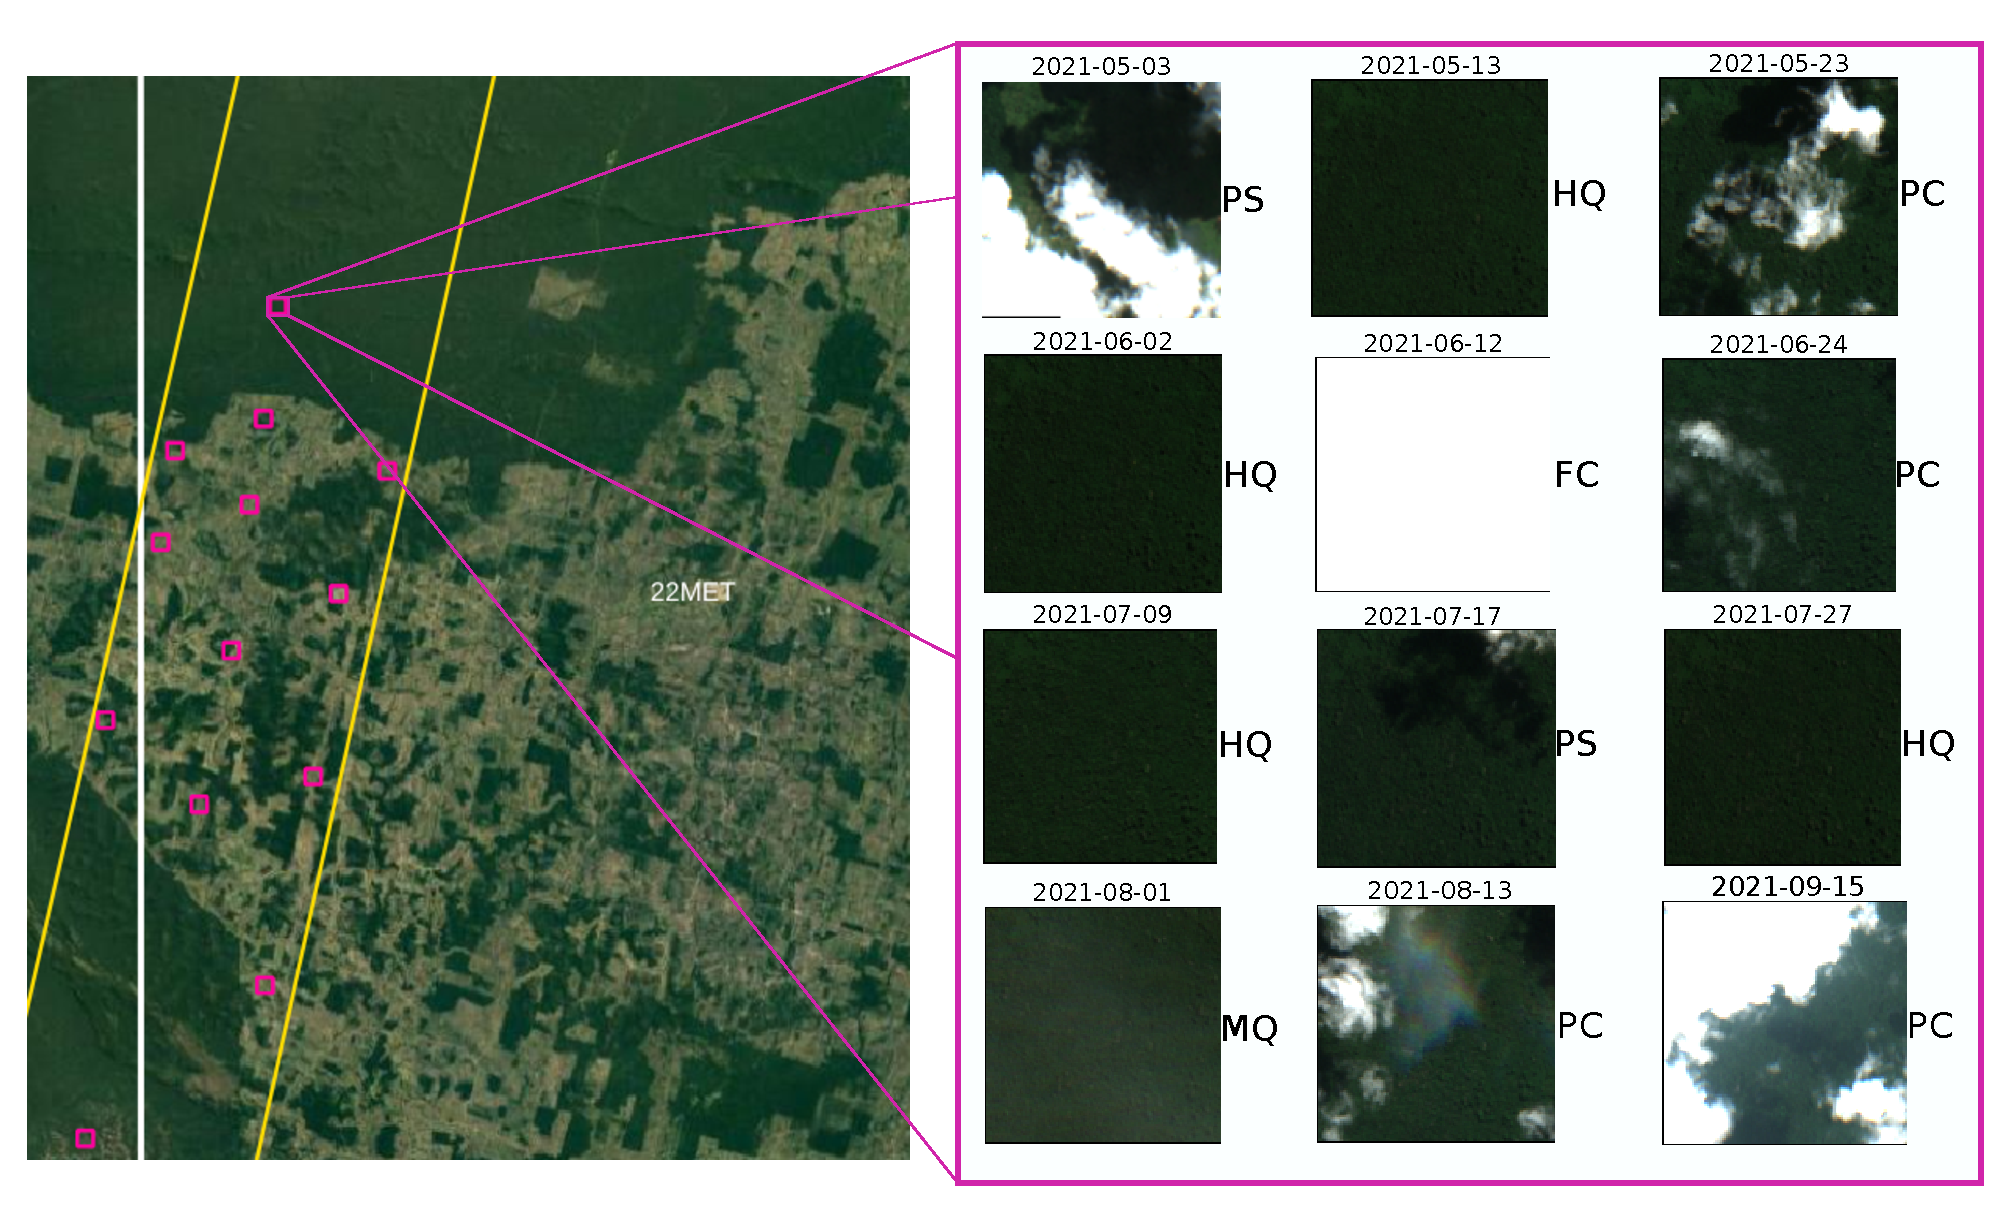
\includegraphics[width=10cm]{Figures/v3/labeling/polygon_11.pdf}
        \caption{Temporal observation of the polygon 11.}  
        \centering
    \end{figure}
\end{frame}

\section{Training}
\begin{frame}{Implementation details}
    \begin{minipage}{0.6\textwidth}
        \begin{table}
            \scriptsize
            \begin{tabular}{c | c} 
                \hline
                Parameter & Value \\ [1ex] 
                \hline
                Training size & 90$\%$ \\ [1ex]
                Testing size & 10$\%$ \\ [1ex]
                Number of observations with HQ & 30 \\
                Classes & 7 \\ [1ex] 
                \hline
            \end{tabular}
        \caption{Dataset split.}
        \end{table}
    \end{minipage}
    \begin{minipage}{0.35\textwidth}
        \begin{table}
            \scriptsize
            \begin{tabular}{c|c}
            \hline
                \multicolumn{2}{c}{Hyperparameters} \\ \hline
                Epochs & 10000 \\ 
                Batch size rate & 0.1* \\ 
                Units in hidden layers & 3 \\ 
                Learning rate & 1e-5 \\ 
                Optimizer & Adam \\ 
                Loss & MSE \\ \hline
                \multicolumn{2}{c}{* of each class}
            \end{tabular}
            \caption{Setting up of the Autoencoders hyperparameters.}
        \end{table}
    \end{minipage}
\end{frame}


\section{Inference}


\section{Thank you}

\end{document}